\section{Implementation}

\subsection{Environment Set-Up}

\subsubsection{Existing Environments}

The first step towards starting the implementation is to set up a
comfortable and adjustable environment. There are several environments
one can use to build Solidity applications, most popular of which are
Truffle(ref), Remix(ref) and Embark(ref). However, none of the
aforementioned applications delivered the experience we needed in the
scope of our project, due to the lack of speed and customization
options. That led us to the creation of a custom environment for
importing, compiling, deploying and testing smart contracts.

We used Python(ref) to build our environment, since it is a powerful
and convenient programming language, and all of our dependencies had
Python implementations available. We developed our environment in
Linux(ref).

\subsubsection{Dependencies}

The components we used as building blocks are Web3(ref) which is a
powerful library for interacting with Ethereum, the Solidity v0.6.6
compiler(ref), and EthereumTester which is a set of tools for testing
Ethereum-based applications. For the purpose of our project, a private
blockchain running an Ethereum Virtual Machine (EVM) was deployed.
This is a common practice for Ethereum developers since it greatly
facilitates testing procedures. Our environment supports multiple
EVMs, namely Geth(ref), Ganache(ref) and Py-EVM(ref).

\subsubsection{Ethereum Virtual Machines}

All aforementioned EVMs deliver an implementation that complies with
the specifications described at the Ethereum yellow paper(ref).
However, different implementations provide unique attributes to the
developer, each of which helped us to progress effortlessly during
different stages of our work.

\paragraph {Py-EVM:} Py-EVM is an evolving EVM which is created mainly for
testing. The ease of access and use, the configuration freedom of its
underlying test chain and its effectiveness for small sized data helped our
first steps. However, as the input data size started to grow, the effectiveness
of the tool rapidly fell(ref).

\paragraph {Ganache:} Ganache is a popular EVM developed by the Truffle team.
It’s speed and configuration freedom are its main advantages. However, its
extreme memory requirement made it impossible to use when the sizes of the
input became analogous to the Bitcoin blockchain size.

\paragraph {Geth:} Geth is another popular EVM which is created by the Ethereum
team. It supports heavy customization while its memory usage is very limited
compared to Ganache, even for extensive inputs. It is, however, slower than
Ganache.

The set of configurations we used for each EVM can be found in our
public repository(ref).

TODO: insert figure of Py-EVM vs Ganache vs Geth

\subsubsection{Gas Profiling}

Another useful utility we used was solidity-gas-profiler(ref), a profiling
utility by Yushih. This gave us great insights regarding the gas usage across
contract’s functions, and, consequently, helped us target the functionalities
that needed to be refined.

TODO: insert figure of gas profiling

\subsection{Model}

As mentioned above, we used a previous verifier implementation(ref) as
a basis for our implementation. Since we adopted common primitives, we
used some of the tools Giorgos et al.\ used for functionalities such as
constructing blockchains and proofs. For the purposes of our project,
we needed to enhance the functionality of the existing tools in some
cases. We are thankful to the writers for sharing their
implementation. This greatly facilitated our work. Similar to Giorgos
et al.\, we follow the steps listed below:

\begin{enumerate}
    \item
        Construct a blockchain
    \item
        Construct a proof for an event in the blockchain
    \item
        Verify the proof
\end{enumerate}

In this subsection, we describe the model under which both
implementations were deployed.

\subsubsection{Blockchain}

The tool that creates the blockchain was created by Andrew Miller, one
of the writers of Non-Interactive Proofs of Proof of Work(ref) paper.
The tool is using the Bitcoin library(ref) to construct a blockchain
similar to Bitcoin’s. The interlink pointers are organised into a
Merkle tree and the index is determined by their level. For details
regarding the level calculation, see section(ref). The Merkle root of
the interlink tree is a 32-bit value, and is included in the
block header as an additional value. The new size of the block header
is 112 bytes. In order to ensure security, it is important for the
interlink root to be included in the block header, as it is part of
the proof. Otherwise, attackers could attack the proofs by reordering
or including stray blocks. Miners can easily verify that the Merkle
root is correct.

TODO: figure of the blockchain

\subsubsection{Superblock Levels}

We assume that the difficulty target of mined blocks is constant. As
discussed in section(ref), this is not the model of the Bitcoin
blockchain. The definition of superblocks is changed to a simpler
definition and the level is determined by the number of leading zeros
of the block header hash. Although this change does not take into
account the difficulty target, the scoring of proof of work does not
generate security holes in the protocol.

\subsubsection{Proof}

The tool that creates proofs was also created by Andrew Miller. The
prover receives the following inputs:

\begin{itemize}
    \item
        A blockchain with interlinks
    \item
        The security parameter k
    \item
        The security parameter m
\end{itemize}

Security parameters k, m are part of the NIPoPoW model and are
explained in section(ref).

The prover’s output is a proof of proof of work that satisfies the
above security parameters. The prover needed to be enhanced in order
to create special test cases (section(ref)) and enable our optimized
architecture (section(ref)).

TODO: figure of proof

\subsubsection{Verifier}

The goal of the verifier is to accept valid proofs and discard invalid
proofs. A proof is submitted in combination with a predicate. The
proof is considered valid if it is constructively correct and the
predicate is true for the chain described by the proof. The predicate
can represent the existence of an event in the source blockchain, such
as the occurrence of a transaction. In our case, the predicate
indicates the existence of a block in the proof.

The verifier functions in two phases: (a) submit phase and (b) contest
phase. Each phase has different inputs and functionalities, and is
performed by different entities.

\paragraph{Submit phase} During the submit phase, an entity submits a
proof and an event. During this phase, we assume that at least one
honest full node is aware of the submission. This is also a part of
the model of NIPoPoW, and is a logical assumption as explained in the
paper. In order to perform a submission, one must provide a proof and
a predicate. If a certain number of rounds passes without contests, the proof
is considered valid and the predicate is considered true. The passing of rounds
is indicated by the mining of new blocks atop of the block containing the
submission.

\paragraph{Contest phase} If the submitted proof is invalid (i.e.\ the
predicate is not true for the honest chain), a contesting proof is
submitted, invalidating the original proof and predicate. The
contesting proof is considered better only if it encapsulates more
proof of work than the existing proof, as described in the NIPoPoWs
paper. In order to contest, one must provide a contest proof and the predicate
that is claimed to be true by the originally submitted proof. If the contesting
proof has better score, then the predicate is evaluated against the contesting
proof.

The correct functionality of the verifier is the following.
\begin{itemize}
    \item
        if an \textit{honest} party submits a proof and no contest occurs, then
        $predicate$ becomes $true$.
    \item
        If an \textit{honest} party submits a proof and it is contested by an
        \textit{adversary}, then the contest is invalid and the $predicate$
        remains $true$.
    \item
        If an \textit{adversary} submits a proof, then an \textit{honest} party
        makes a contest. The contest invalidates the original submission and
        the $predicate$ becomes $false$.
    \item
        The scenario in which an \textit{adversary} submits a proof and it is not
        followed by an \textit{honest} contest cannot take place due to the assumption
        that at least one honest party observes the traffic of the contract.
\end{itemize}

\subsection{Previous Implementation}

In this subsection we present previous work. We prepare the reader by focusing
at specific aspects in which our solution differs. We will later show these
differences and we will analyse on how they impact the results of our
application.

\subsubsection{Overview}
As mentioned in the NIPoPoWs(ref Algorithm 7) paper, in order to construct a
verifier, a DAG structure needs to be maintained in memory. This structure is
stored in the form of a hashmap, and is used to host blocks of all different
proofs. This process aims to prevent adversarial proofs which are structurally
valid, but blocks are intentionally skipped. Such a scenario is displayed in
Figure~\ref{fig:DAG_usage}. The DAG is used to construct ancestors structure.
By iterating ancestors, we can securely determine the value of the predicate.

\begin{figure}[hbt]
    \centering
    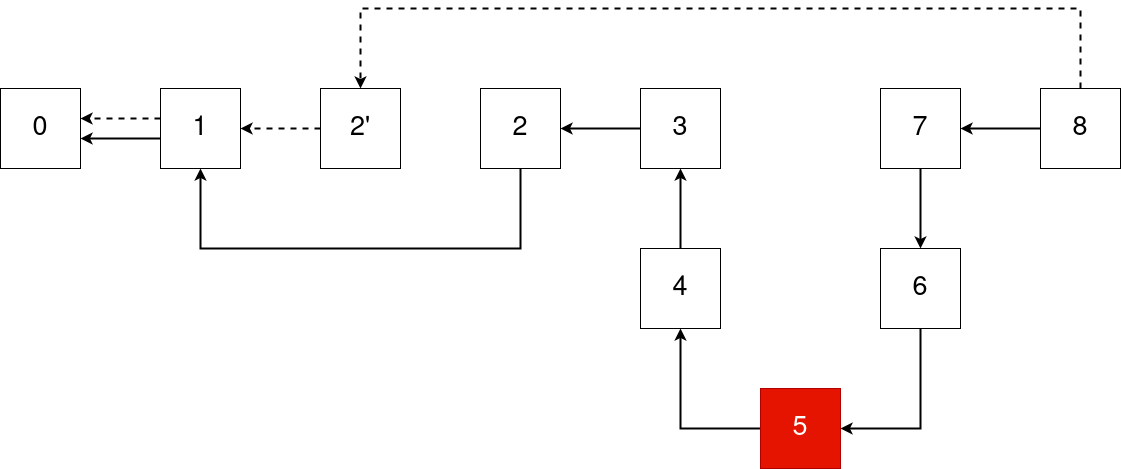
\includegraphics[width=10cm]{DAG_usage}
    \caption{Combination of multiple proofs in a DAG. The red block is the
        block of interest. Solid proof consists of blocks connected by solid
        lines and adversary proof by dashed lines.The adversary intentionally
        uses a different set of blocks.}
    \label{fig:DAG_usage}
\end{figure}

This logic is intuitive and efficient to implement in most traditional
programming languages (C++, JAVA, Python, JavaScript, etc). However, such an
algorithm cannot be efficiently implemented in Solidity as is. This is not
due to the lack of features, such as the existence of hashmaps, but because
Solidity treats storage differently than most programming languages. As
mentioned above(ref) in smart contracts the caller needs to pay in gas the
execution of operations such as accessing and storing data. Reading from and
writing to persistent memory are very expensive operations in Solidity, as
stated in the Ethereum yellow paper(ref). A summary of gas costs is displayed
in Figure~\ref{fig:gas_prices}. This fact was observed by Giorgos et al.\ and
was recognized as the bottleneck of the application.

\begin{figure}[hbt]
    \centering
    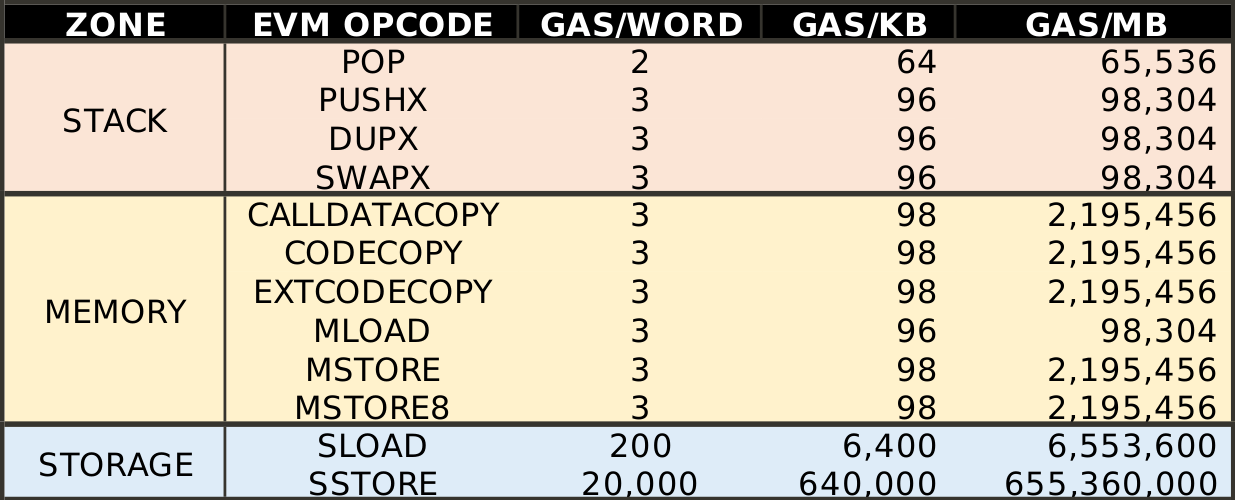
\includegraphics[width=12cm]{gas_prices}
    \caption{Gas prices per operation.}
    \label{fig:gas_prices}
\end{figure}

\subsubsection{Phases}

We describe each phase of the previous implementation in
Algorithms~\ref{algo:submit_old} and~\ref{algo:contest_old}. We highlight
structures that access persistent memory. Note that deleting from persistent
memory is also considered a storage operation

\begin{algorithm}
    \caption{Submit Event Proof}
    \label{algo:submit_old}
    \KwIn{$proof$, $predicate$}
    \KwData{
        \texttt{array} $proof_{s}$,
        \texttt{hashmap} $DAG_{s}$,
        \texttt{bool} $predicate_{s}$
    }
    require $predicate_{s}$ $=$ $\emptyset$ \\
    require $validInterlink(proof$) \\
    $DAG_{s}$ $\leftarrow$ $DAG_{s}$ $\cup$ $proof$\\
    $proof_{s}$ $\leftarrow$ $proof$\\
    $ancestors_{s}$ $\leftarrow$ $findAncestors(DAG_{s}$)\\
    $predicate_{s}$ $\leftarrow$ $evaluatePredicate(ancestors_{s}$,
    $predicate$)\\
    delete $ancestors_{s}$\\
\end{algorithm}

\begin{algorithm}
    \caption{Submit Contesting Proof}
    \label{algo:contest_old}
    \KwIn{$proof'$, $predicate$}
    \KwData{
        \texttt{array} $proof_{s}$,
        \texttt{hashmap} $DAG_{s}$,
        \texttt{bool} $predicate_{s}$
    }
    require $predicate_{s}$ = $predicate$\\
    $lca$ $\leftarrow$ findLca($proof_{s}$, $proof'$)\\
    require $score(proof’[lca:])$ $>$ $score(proof_{s}[lca:])$ \\
    $DAG_{s}$ $\leftarrow$ $DAG_{s}$ $\cup$ $proof'$\\
    $ancestors_{s}$ $\leftarrow$ $findAncestors(DAG_{s})$\\
    $predicate_{s}$ $\leftarrow$ $evaluatePredicate(ancestors_{s},
    predicate)$\\
    delete $ancestors_{s}$\\
\end{algorithm}

\subsubsection{Security analysis}

\paragraph{Pre-mining}
We observed that the smart contract is vulnerable to pre-mining(ref). By
definition, a valid NIPoPoW is considered structurally correct if two
properties are satisfied:

\begin{enumerate}[(a)]

\item The interlink structure of all blocks is correct. This is to prevent
    adversaries from injecting blocks that do not exist in the original
    blockchain.

\item The first block of proof is $genesis$. This is to prevent adversaries
    from create coins before blockchain was initiated in the public network.

\end{enumerate}

The second property is not verified in the smart contract, exposing it to
pre-mining attacks. We can easily mitigate this vulnerability by initializing
the smart contract with the $genesis$ block of the blockchain we will use to
create proofs, and add an assertion that submitted proofs satisfy property (b).
We needed changes are shown in Algorithms~\ref{algo:avoid_premining_ctor}
and~\ref{algo:avoid_premining_submit}.

\begin{algorithm}
    \caption{Constructor}
    \label{algo:avoid_premining_ctor}
    \KwIn{$genesis$ block}
    $genesis_{s}$ $\leftarrow$ $genesis$
\end{algorithm}
\vspace{-0.7cm}
\begin{algorithm}
    \caption{Submit Event Proof}
    \label{algo:avoid_premining_submit}
    \KwIn{$proof$, ...}
    require $proof[0]$ = $genesis_{s}$ \\
    ...
\end{algorithm}


\subsubsection{Gas analysis}
\subsection{Targeting vulnerabilities and costly functionalities}

\begin{itemize}
    \item
        0. Knowledge that extensive gas usage is due to large storage
        allocation
    \item
        1. Make old contract compatible with the last version of solidity
        compiler
    \item
        2. Create tests for all functionalities
    \item
        3. Identify and fix vulnerabilities
\begin{figure}
    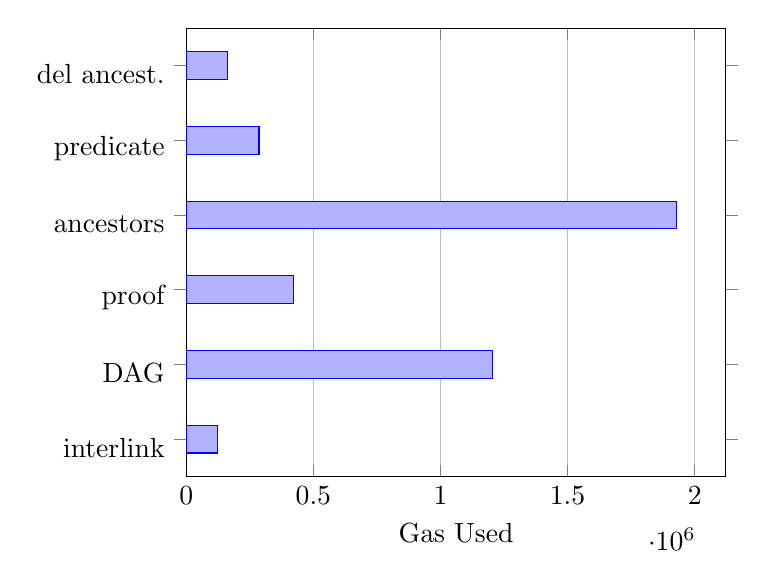
\begin{tikzpicture}
        \begin{axis}[
            symbolic y coords={
                interlink,
                DAG,
                proof,
                ancestors,
                predicate,
                del ancest.
            },
            ytick={interlink, DAG, proof, ancestors, predicate, del ancest.},
            yticklabel style={text height=3ex},
            xmin=0,
            xbar,
            xlabel={Gas Used},
            xmajorgrids=true,
            ]
            \addplot coordinates {
                    (124208,interlink)
                    (1204142,DAG)
                    (422535,proof)
                    (1929705,ancestors)
                    (286295,predicate)
                    ( 163696,del ancest.)
                };
        \end{axis}
    \end{tikzpicture}
    \caption{Operations gas cost on submit}
    \label{fig:submit_old_gases}
\end{figure}

\begin{figure}
    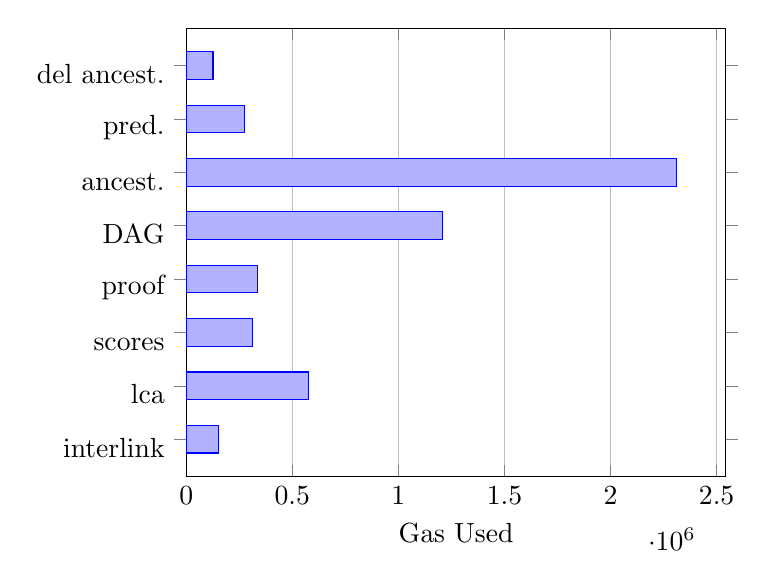
\begin{tikzpicture}
        \begin{axis}[
            symbolic y coords={
                interlink,
                lca,
                scores,
                proof,
                DAG,
                ancest.,
                pred.,
                del ancest.
            },
            ytick={
                interlink,
                lca,
                scores,
                proof,
                DAG,
                ancest.,
                pred.,
                del ancest.
            },
            yticklabel style={text height=3ex},
            xmin=0,
            xbar,
            xlabel={Gas Used},
            xmajorgrids=true,
            ]
            \addplot coordinates {
                    (151715,interlink)
                    (574156,lca)
                    (313897,scores)
                    (337815,proof)
                    (1208754,DAG)
                    (2312361,ancest.)
                    (272718,pred.)
                    (126153,del ancest.)
                };
        \end{axis}
    \end{tikzpicture}
    \caption{Operations gas cost on contest}
    \label{fig:contest_old_gases}
\end{figure}

        Contract is vulnerable to pre-mining
    \item
        4. Profile contract gas usage
    \item
        5. Identify expensive operations
\end{itemize}

\subsection{Fixing vulnerabilities and restricting gas usage}

\begin{itemize}

    \item
        Add verification of genesis
    \item
        Reconsider DAG and ancestors methodology and redesign submission and
        contest schema
    \item
        Submit doesn't need to save in the proof in storage. Contest can
        provide the existing proof during contesting.

    \item
        Use subset: P1\{:lca\} $>$ P2\{:lca\}, P1 is the existing, P2 is the
        contesting

        This prevents expensive storage for DAG and ancestors.

    \item
        Even the check of subset can be skipped. The contesting proof cannot
        benefit from pre-lca malformed proof. If Pa is valid, then we just
        need to check Pb[lca:]

    \item
        This is not vulnerable to DOS attacks

    \item
        Observe the network and contest with the appropriate proof if
        submitted is not correct.

\end{itemize}

\pagebreak
